\documentclass[spanish, 10pt,a4paper]{article}
\usepackage[spanish]{babel}
\usepackage[utf8]{inputenc}
\usepackage{textcomp}
\usepackage{hyperref}
\usepackage[pdftex]{graphicx}
\usepackage{epsfig}
\usepackage{amsmath}
\usepackage{hyperref}
\usepackage{amssymb}
\usepackage{color}
\usepackage{graphics}
\usepackage{amsthm}
\usepackage{subcaption}
\usepackage{caratula}
\usepackage{fancyhdr,lastpage}
\usepackage[paper=a4paper, left=1.4cm, right=1.4cm, bottom=1.4cm, top=1.4cm]{geometry}
\usepackage[table]{xcolor} % color en las matrices
\usepackage[font=small,labelfont=bf]{caption} % caption de las figuras en letra mas chica que el texto
\usepackage[ruled,vlined,linesnumbered]{algorithm2e}
\usepackage{listings}
\usepackage{float}
\usepackage{pdfpages}
\usepackage{amsfonts}


\color{black}

%%%PAGE LAYOUT%%%
\topmargin = -1.2cm
\voffset = 0cm
\hoffset = 0em
\textwidth = 48em
\textheight = 164 ex
\oddsidemargin = 0.5 em
\parindent = 2 em
\parskip = 3 pt
\footskip = 7ex
\headheight = 20pt
\pagestyle{fancy}
\lhead{IS1 - Trabajo Pr\'actico 1} % cambia la parte izquierda del encabezado
\renewcommand{\sectionmark}[1]{\markboth{#1}{}} % cambia la parte derecha del encabezado
\rfoot{\thepage}
\cfoot{}
\numberwithin{equation}{section} %sets equation numbers <chapter>.<section>.<subsection>.<index>

\newcommand{\figurewidth}{1\textwidth}

\newcommand{\tuple}[1]{\ensuremath{\left \langle #1 \right \rangle }}
\newcommand{\Ode}[1]{\small{$\mathcal{O}(#1)$}}


%El siguiente paquete permite escribir la caratula facilmente
\hypersetup{
  pdftitle={ IS1 - TP1 },
  colorlinks,
  citecolor=black,
  filecolor=black,
  linkcolor=black,
  urlcolor=black 
}

\materia{Ingeniería de Software I}

\titulo{Trabajo Práctico 1}

\subtitulo{Informe y diagramas.}

\grupo{Grupo 2}

\integrante{De Sousa Bispo, Germán}{359/12}{germandesousa@gmail.com}
\integrante{Fernandez, Esteban}{691/12}{esteban.pmf@gmail.com}
\integrante{Kodelia, Erika Natasha}{767/11}{erikankodelia@gmail.com}
\integrante{Mongi Badia, Martín}{422/13}{martinmongi@gmail.com}
\integrante{Sánchez Cano, Gonzalo}{}{xeneize__86@hotmail.com}
\integrante{Wright, Carolina}{876/12}{wright.carolina@gmail.com}

 
\begin{document}
{ \oddsidemargin = 2em
	\headheight = -20pt
	\maketitle
}
	
\section{Introducción}
	El Ministro de Gobierno quiere modificar el Sistema Electoral Nacional y para ello propone instalar en las escuelas máquinas emisoras de sufragios. Junto con esta incorporación se deberá modificar el Sistema del Centro de Cómputos Nacional para que pueda operar con las máquinas.

	El formato de la votación no presenta cambios, es decir, al igual que en el sistema de boletas que se venía utilizando se permitirá votar por categorías o votar en blanco. 
	
	Además se busca proveer todos los mecanimos necesarios para asegurar el derecho de voto a todos los Electores. Se considerarán las necesidades de los no videntes y personas con movilidad reducida.
	
\subsection{Técnicas de Especificación}

En este Trabajo Práctico, se nos pide especificar varios aspectos de el Sistema que pretendemos construir:
\vspace{-2em}
\paragraph{Diagrama de contexto:} Un diagrama de contexto es una vista del sistema en la cual se especifican todas las interacciones que el Sistema debe tener con todos los agentes exteriores al mismo. El diagrama es un multigrafo dirigido, en el cual uno de los nodos es el sistema y el resto son los agentes que interactuarán con este. Las interacciones son representadas por los ejes dirigidos del mismo, los cuales se etiquetan con la acción que representan. Es útil para ver todas las acciones que uno debiera preveer e implementar en el Sistema, y también ver que interacciones no pertenecen al Sistema y por ende no es necesaria su implementación. Es importante destacar que este tipo de vista no provee información sobre el funcionamiento interno del Sistema, ya que se trata de una vista de alto nivel.
\paragraph{Diagrama de objetivos:} Un diagrama de objetivos es una vista en el sistema en la cual se especifican los objetivos del Sistema en todos sus niveles. En este diagrama, se empieza con un nodo raíz, que es el objetivo duro general a satisfacer, y se van refinando estos objetivos. Estos refinamientos pueden ser de dos tipos: o-refinamiento e y-refinamiento. El primero modela un objetivo para el cual se necesita que todos los objetivos que contribuyen a este se cumplan para cumplirse. El segundo modela un objetivos para el cual con que se cumpla uno de los subobjetivos que contribuyen a este se cumpla para cumplirse. Este último cobra relevancia con el agregado de los objetivos blandos. Los objetivos son blandos cuando sólo es posible establecer un orden entre dos o más alternativas. Un ejemplo de esto sería cuando se desea que un Sistema sea barato: el costo de un Sistema sólo puede usarse para comparar dos o más alternativas. Los o-refinamientos permiten en este caso, explicar las diferentes alternativas de implementación con sus pros y contras. Finalmente, cuando se ha conseguido un refinamiento en los objetivos operacionales y el diagrama tiene la granularidad necesaria, se asigna cada objetivo a un agente externo o al Sistema a implementar. De esta forma, es mucho más fácil designar que es un requerimiento del Sistema y que es un objetivo en el que influirá un agente externo.
\vspace{1em}

También, se nos pidió efectuar una especificación informal de los escenarios de uso del Sistema. De esta forma, se explica a alto nivel, como el futuro usuario debera interactuar con el Sistema.
	
\section{Requerimientos}
\begin{itemize}
\item Lograr que el CCN almcene internamente conteos parciales y totales.
\item Lograr implementar una interfaz Web del CCN para proveer resultados parciales y totales a la página Web.
\item Lograr que el CCN brinde información de los candidatos cuando la página web lo solicite.
\item Lograr que el CCN permita cargar el padrón de electores.
\item Lograr implementar una interfaz Web del CCN para proveer el padrón a la página web.
\item Lograr que el CCN permita almacenar el padrón internamente.
\item Lograr que la máquina emisora de sufragios permita modo \emph{root} mediante boletas especiales.
\item Lograr calcular mediante porcentajes (sin sistema D'Hondt) gobernadores, presidentes, etc. electos totales y parciales.
\item Lograr calcular mediante método D'Hondt diputados electos totales y parciales.
\item Lograr que la CCN reciba los sufragios y conteos parciales de los servidores locales.
\item Lograr considerar un voto emitido al momento de la confirmación del voto.
\item Lograr que los servidores locales reciban los sufragios de las máquina emisoras.
\item Lograr que los servidores locales envíen los conteos parciales y votos al CCN en rangos de 30 minutos.
\item Lograr que el CCN al actualizar los conteos parciales, actualice los conteos totales.
\item Lograr que el CCN reciba los conteos manuales parciales de los colegios.
\item Lograr que el servidor local de cada escuela almacene los votos manuales ingresados por cada presidente de mesa en la máquina de sufragios de su correspondiente mesa.
\item Lograr que las máquinas de sufragios reciban, mientras en modo \emph{root}, los conteos manuales.
\item Lograr que los servidores locales envíen los conteos manuales de sus mesas al CCN.
\item Lograr que el CCN verifique correspondencia entre los conteos manuales y los electrónicos.
\item Lograr que el CCN actualice su base de información de votos y diferencias, para proveer a la página web.
\item Lograr que la máquina emisora de sufragios permita el acceso solamente cuando una boleta válida es introducida.
%\item Lograr que la máquina emisora de sugragios permita seleccionar el partido al que se quiere votar.
%\item Lograr que al seleccionar el partido, la máquina permita seleccionar el candidato al que se quiere votar.
\item Lograr variar la ubicación de los partidos y candidatos en la pantalla. ¿¿CAMBIAR POR OBJETIVOS BLANDOS??
\item Lograr proveer información sobre partidos y candidatos a través de Internet, desde el CCN.
\item Lograr que la máquina de sufragios obtenga la información sobre partidos y candidatos del CCN.
\item Lograr que la máquina de sufragios provea información sobre los candidatos y partidos al elector.
\item Lograr permitir el voto por categorías.
\item Lograr permitir votar la lista completa.
\item Lograr permitir votar en blanco.
\item Lograr habilitar y deshabilitar las máquinas emisoras de sufragios, mediante la boleta de acceso \emph{root}.
\item Lograr que la máquina de sufragios confirme el voto al realizarlo.
\item Lograr que la máquina de sufragios imprima el voto al confirmarlo.
\item Lograr que la máquina de sufragios permita ingresar la boleta.
\item Lograr que la máquina de sufragios autentique al elector a través de la huella dactilar.
\item Lograr que la máquina de sufragios permita emitir el sufragio, al ingresar la boleta.
\item Lograr que la máquina de sufragios permita emitir el sufragio a través del audio.

\end{itemize}

\section{Hipótesis de dominio}

\begin{itemize}
\item Sólo votan los electores discapacitados sin declaración judicial de incapacidad.
\end{itemize}

\section{Diagrama de objetivos}

En el diagrama de objetivos entregado previamente, no habíamos explicado correctamente la difusión de los resultados parciales de la elección. Nos referimos a esta rama de objetivos:

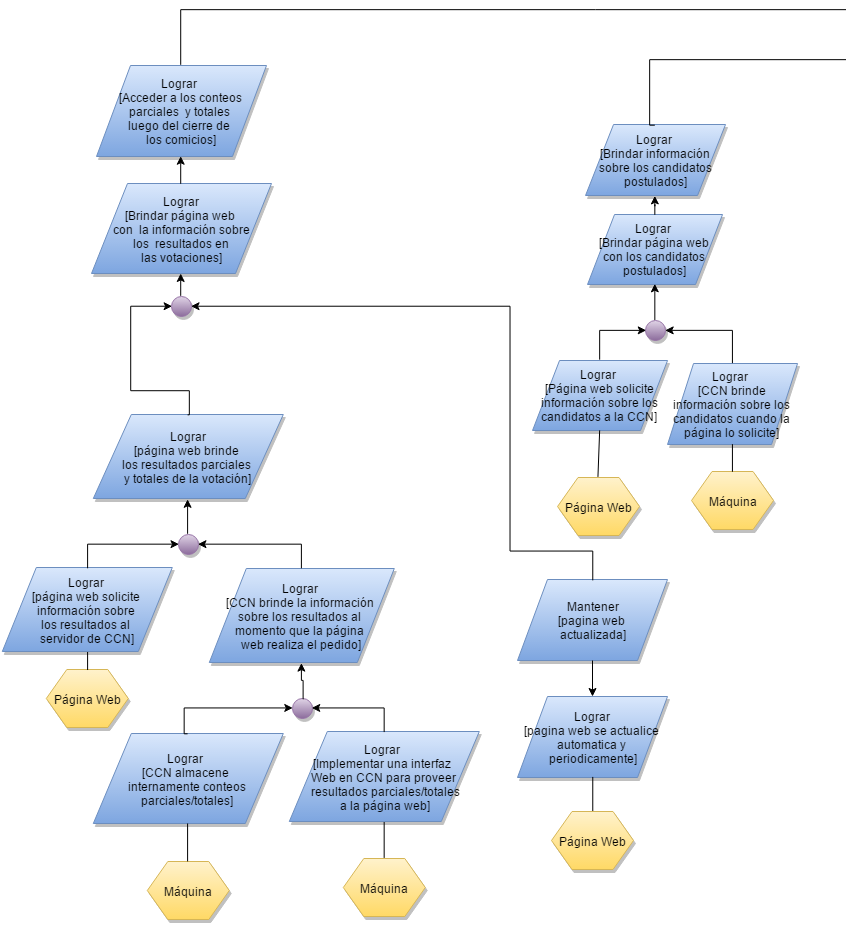
\includegraphics[width=\textwidth]{diagrama.png}

En este diagrama, ``Lograr que la página web brinde resultados parciales y totales de la votación'' significa que, pasabas las 18 horas, la página web empiece a mostrar los resultados de las votaciones mientras se van sumando los votos de los diferentes candidatos. No implica que se conozcan antes de las 18 horas, ya que dicha difusión sería ilegal..
\end{document}
